
%(BEGIN_QUESTION)
% Copyright 2010, Tony R. Kuphaldt, released under the Creative Commons Attribution License (v 1.0)
% This means you may do almost anything with this work of mine, so long as you give me proper credit

Denne analoge elektroniske regulator-kretsen har et problem. Utgangssignalet er mettet over 100\% uansett hvilke signaler som mates inn på PV-terminalen, og uansett hvor SP justeres:

$$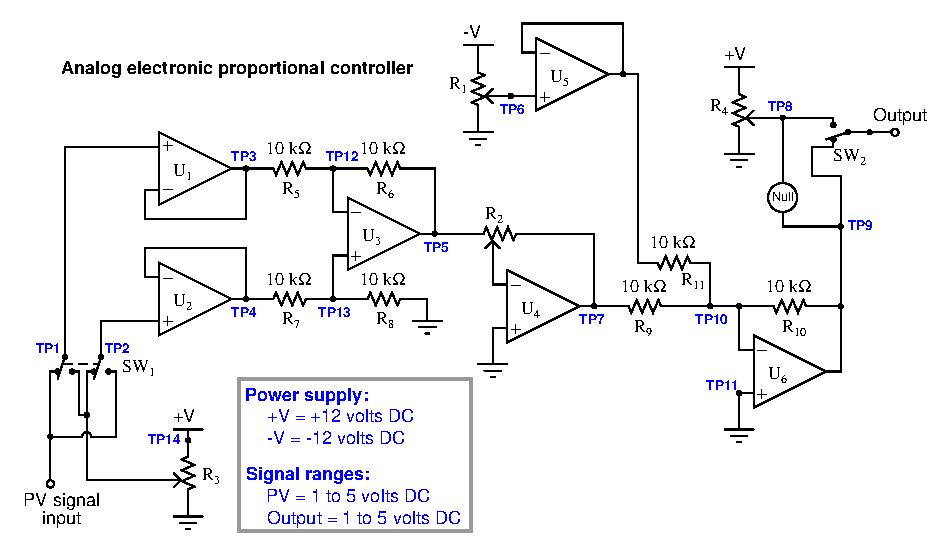
\includegraphics[width=15.5cm]{i01416x01.eps}$$

Med PV-inngangssignal på +3.00 volt og settpunktsignal på +2.58 volt måler en tekniker $-0.42$ volt DC ved testpunkt TP5. Vurder sannsynligheten for hver spesifisert feil i denne kretsen. Vurder hver feil separat (det vil si ingen samtidige feil), og avgjør om hver enkelt feil alene kan forklare {\it alle} målinger og symptomer i kretsen.

% No blank lines allowed between lines of an \halign structure!
% I use comments (%) instead, so that TeX doesn't choke.

$$\vbox{\offinterlineskip
\halign{\strut
\vrule \quad\hfil # \ \hfil & 
\vrule \quad\hfil # \ \hfil & 
\vrule \quad\hfil # \ \hfil \vrule \cr
\noalign{\hrule}
%
% First row
{\bf Feil} & {\bf Mulig} & {\bf Umulig} \cr
%
\noalign{\hrule}
%
% Another row
Opamp $U_1$ utgang feilet mot lav rail &  &  \cr
%
\noalign{\hrule}
%
% Another row
Opamp $U_4$ utgang feilet mot høy rail &  &  \cr
%
\noalign{\hrule}
%
% Another row
Opamp $U_5$ utgang feilet mot lav rail &  &  \cr
%
\noalign{\hrule}
%
% Another row
$R_1$-forbindelse til jord feilet åpen &  &  \cr
%
\noalign{\hrule}
%
% Another row
$R_3$-forbindelse til +V feilet åpen &  &  \cr
%
\noalign{\hrule}
%
% Another row
Motstand $R_8$ feilet åpen &  &  \cr
%
\noalign{\hrule}
%
% Another row
Motstand $R_9$ feilet åpen &  &  \cr
%
\noalign{\hrule}
%
% Another row
Motstand $R_{10}$ feilet åpen &  &  \cr
%
\noalign{\hrule}
%
% Another row
Motstand $R_{11}$ feilet åpen &  &  \cr
%
\noalign{\hrule}
} % End of \halign 
}$$ % End of \vbox

Til slutt: Angi den {\it neste} diagnostiske testen eller målingen du ville gjort på dette systemet. Forklar hvordan resultatet av denne neste testen/målingen hjelper deg videre med å identifisere feilens plassering og/eller natur.

\vskip 20pt \vbox{\hrule \hbox{\strut \vrule{} {\bf Forslag til sokratisk diskusjon} \vrule} \hrule}

\begin{itemize}
\item{} Beregn riktig posisjon for potensiometer $R_1$ for å sette regulatorens bias-verdi til 50\%.
\end{itemize}

\underbar{file i01416}
%(END_QUESTION)





%(BEGIN_ANSWER)

% No blank lines allowed between lines of an \halign structure!
% I use comments (%) instead, so that TeX doesn't choke.

$$\vbox{\offinterlineskip
\halign{\strut
\vrule \quad\hfil # \ \hfil & 
\vrule \quad\hfil # \ \hfil & 
\vrule \quad\hfil # \ \hfil \vrule \cr
\noalign{\hrule}
%
% First row
{\bf Feil} & {\bf Mulig} & {\bf Umulig} \cr
%
\noalign{\hrule}
%
% Another row
Opamp $U_1$ utgang feilet mot lav rail &  & $\surd$ \cr
%
\noalign{\hrule}
%
% Another row
Opamp $U_4$ utgang feilet mot høy rail &  & $\surd$ \cr
%
\noalign{\hrule}
%
% Another row
Opamp $U_5$ utgang feilet mot lav rail & $\surd$ &  \cr
%
\noalign{\hrule}
%
% Another row
$R_1$-forbindelse til jord feilet åpen & $\surd$ &  \cr
%
\noalign{\hrule}
%
% Another row
$R_3$-forbindelse til +V feilet åpen &  & $\surd$ \cr
%
\noalign{\hrule}
%
% Another row
Motstand $R_8$ feilet åpen &  & $\surd$ \cr
%
\noalign{\hrule}
%
% Another row
Motstand $R_9$ feilet åpen & ? &  \cr
%
\noalign{\hrule}
%
% Another row
Motstand $R_{10}$ feilet åpen & ? &  \cr
%
\noalign{\hrule}
%
% Another row
Motstand $R_{11}$ feilet åpen &  & $\surd$ \cr
%
\noalign{\hrule}
} % End of \halign 
}$$ % End of \vbox

$R_1$-forbindelse til jord feilet åpen er mulig fordi dette potensiometeret er koblet til negativ forsyningsskinne (-V), og en åpen jordforbindelse vil derfor gjøre bias-signalet fullt negativt, noe som driver regulatorens utgang fullt positiv.

\vskip 10pt

Åpen $R_9$ eller åpen $R_{10}$ gir kun mening for visse (store) bias-verdier, dersom utgangen aldri avviker fra full metning {\it uansett hvilke verdier som mates inn på PV eller SP}.

%(END_ANSWER)





%(BEGIN_NOTES)

En god ``neste test'' vil være å måle utgangen fra neste opamp-trinn (TP7) for å se om signalet fortsatt ``gir mening'' der også, siden signalet vi målte på TP5 var riktig (forskjellen mellom PV og SP).





\filbreak \vskip 20pt \vbox{\hrule \hbox{\strut \vrule{} {\bf Virtuell feilsøking} \vrule} \hrule}

\noindent
{\bf Forutsi effekten av en gitt feil:} presenter hver av følgende feil for studentene, én om gangen, og la dem kommentere alle effekter hver feil vil gi.

\begin{itemize}
\item{} Motstand $R_5$ feiler åpen
\item{} Motstand $R_6$ feiler åpen
\item{} Motstand $R_7$ feiler åpen
\item{} Motstand $R_8$ feiler åpen
\item{} Motstand $R_9$ feiler åpen
\item{} Motstand $R_{10}$ feiler åpen
\item{} Motstand $R_{11}$ feiler åpen
\item{} TP5 kortsluttes til jord 
\item{} TP6 kortsluttes til jord 
\item{} TP7 kortsluttes til jord 
\item{} TP8 kortsluttes til jord 
\item{} Nullvoltmeter feiler åpen
\item{} Opamp $U_1$ feiler med lav utgang
\item{} Opamp $U_3$ feiler med høy utgang
\item{} Opamp $U_4$ feiler med lav utgang
\item{} Opamp $U_5$ feiler med høy utgang
\end{itemize}


\vskip 10pt


\noindent
{\bf Identifiser mulige/umulige feil:} presenter symptomer for studentene, og la dem deretter avgjøre om en serie foreslåtte feil kan forklare alle symptomene, med forklaring av {\it hvorfor} eller {\it hvorfor ikke} for hver foreslått feil:

\begin{itemize}
\item{} Symptom: {\it }
\item{} 
\item{} 
\item{} 
\end{itemize}


\vskip 10pt


\noindent
{\bf Vurder nytten av foreslåtte diagnostiske tester:} presenter symptomer for studentene og foreslå så følgende diagnostiske tester én etter én. Studentene vurderer verdien av hver test, og avgjør om testen gir nyttig informasjon (det vil si forteller oss noe vi ikke allerede vet). Studentene avgjør også hva ulike resultater av hver test kan indikere om feilen, om noe:

\begin{itemize}
\item{} Symptom: {\it }
\item{}  -- {\bf Ja/Nei}
\item{}  -- {\bf Ja/Nei}
\end{itemize}


\vskip 10pt


\noindent
{\bf Diagnostiser en feil basert på gitte symptomer:} forestill deg at ??? feiler ??? i dette systemet (ikke avslør feilen til studentene!). Presenter operatørens observasjon(er) for studentene, la dem vurdere mulige feil og diagnostiske strategier, og oppgi deretter resultatene av testene de foreslår basert på symptomene under, helt til de har identifisert feilens natur og plassering korrekt:

\begin{itemize}
\item{} {\it }
\item{} 
\item{} 
\end{itemize}
%INDEX% Control, proportional: analog electronic controller

%(END_NOTES)

